\documentclass[parskip]{scrartcl}
\usepackage[margin=15mm]{geometry}
\usepackage{tikz}
\usetikzlibrary{calc,intersections,through,backgrounds}

\begin{document}

\begin{tikzpicture}
    \coordinate (A) at (0,0);
    \coordinate (B) at (3,3);
    \draw [name path=A--B] (A) -- (B);
    \coordinate (C) at (3,0);
    \coordinate (D) at (0,1);
    \draw [name path=C--D] (C) -- (D);
    \path [name intersections={of=A--B and C--D,by=E}];
    \node [fill=red,inner sep=1pt,label=-90:$E$] at (E) {};
\end{tikzpicture}



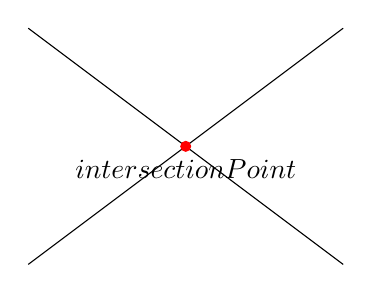
\begin{tikzpicture}
    \draw[name path=line1] (0, 0) -- (4, 3);
    \draw[name path=line2] (4, 0) -- (0, 3);

    \path[name intersections={of=line1 and line2, by={intersectionPoint}}];

    \fill[red] (intersectionPoint) circle (2pt);
    \node [fill=red,inner sep=1pt,label=-90:$intersectionPoint$] at (intersectionPoint) {};

    % \node at (intersectionPoint) {Intersection};
\end{tikzpicture}

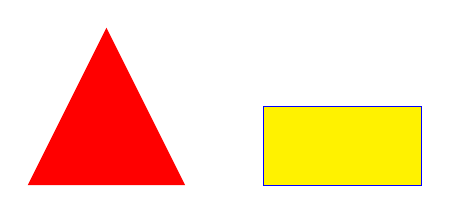
\begin{tikzpicture}
    \fill[red] (0, 0) -- (2, 0) -- (1, 2) -- cycle;
    \filldraw[blue, fill=yellow] (3, 0) rectangle (5, 1);
\end{tikzpicture}

\begin{tikzpicture}
    % Draw the rectangle
    \draw (0,0) rectangle (3,2);

    % Add characters at each corner
    \node[anchor=south east] at (0,0) {A}; % Bottom-left
    \node[anchor=south west] at (3,0) {B}; % Bottom-right
    \node[anchor=north west] at (3,2) {C}; % Top-right
    \node[anchor=north east] at (0,2) {D}; % Top-left
\end{tikzpicture}

\end{document}